\documentclass[11pt,letterpaper]{article}
\usepackage[lmargin=1in,rmargin=1in,bmargin=1in,tmargin=1in]{geometry}
\usepackage{style}

\setlength{\parindent}{0ex}

% -------------------
% Content
% -------------------
\begin{document}

\begin{center}
{\bfseries\Large Elliptic Tales:} \par 
{\bfseries\large A Story of Bitcoin, Moonshine, String Theory, and Clocks} \pspace
{\bfseries\large March 14, 2025} \par\vspace{1cm}
{\large \bfseries Reference Sheet}
\end{center}

\begin{itemize}
\item {\bfseries Arithmetic Geometry.} Broadly speaking, arithmetic geometry is essentially the study of `nice solutions' to `nice equations.' What is typically meant by this is Diophantine equations, i.e. integer solutions to equations in polynomials with integer coefficients. However, the term is often meant broader to systems of equations in polynomials with coefficients coming from rings with a lot of `interesting arithmetic structure.'

\item Common questions asked in the study of equations to arithmetic geometers: are there integer, rational, etc. solutions to an equation, if there are solutions then how many, can we find the solutions, can we describe (parametrize) the solutions, can we find an algorithm to compute all the solutions, etc. 

 \begin{thm*}[Rational Roots Theorem]
Let $f(x)= a_n x^n + a_{n-1} x^{n-1} + \cdots + a_0$, where $a_i \in \Z$ and $a_0,a_n \neq 0$. Then the only rational solutions to $f(x)=0$ have $x= p/q$, where $p$ is an integer factor of $a_0$ and $q$ is an integer factor of $a_n$. 
\end{thm*}

\begin{thm*}[Linear Diophantine Equations in Two Variables]
Let $a, b, c$ be integers with $a, b \neq 0$ and let $d= \gcd(a, b)$. The equation $ax + by= c$ has integer solutions if and only if $d \mid c$. If so, the equation has infinitely many solutions and all solutions have the form\dots
	\[
	x= x_0 + \frac{b}{d} \, k, \quad y= y_0 - \frac{a}{d} \, k,
	\]
where $(x_0, y_0)$ is a solution and $k$ is an integer. 
\end{thm*}

\item {\bfseries Finding Rational Points on Conics.} If there is a rational point on a conic section, we can find all the rational points on the conic and parametrize them all (except one) by `projecting' this point onto a line. Take the rational parametrization of the circle $x^2 + y^2= 1$ using the point $(-1, 0)$ as our rational point and projecting onto the $y$-axis (the line $x= 0$); that is, connect $(-1, 0)$ to a point $(0, t)$ on the line $x= 0$ using a line, where $t \in \mathbb{Q}$.
	\[
	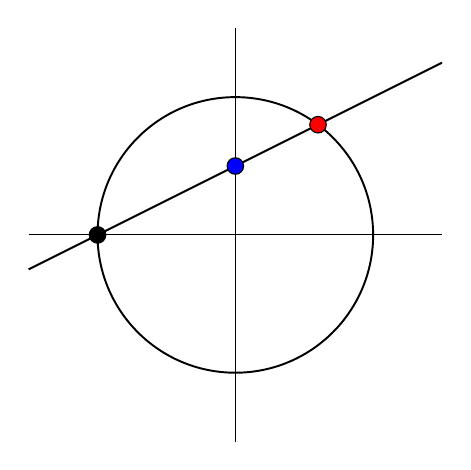
\begin{tikzpicture}[scale=1.75]
	\draw (-1.5,0) -- (1.5,0);
	\draw (0,-1.5) -- (0,1.5);

	\draw[line width=0.7] (-1.5,-0.25) -- (1.5,1.25);
	\draw[line width=0.7] (0,0) circle (1);
	
	\draw[fill=black] (-1,0) circle (0.06);
	\draw[fill=blue] (0,0.5) circle (0.06);
	\draw[fill=red] (0.6,0.8) circle (0.06);
	\end{tikzpicture}
	\] \vfill
	\[
	C(\Q)= \{ (-1,0) \} \cup \left\{ \left(\dfrac{1-t^2}{1+t^2}, \dfrac{2t}{1+t^2} \right) \colon t \in \Q \right\}
	\]

\begin{prin}[Hasse, Local-Global Principle]
A collection of equations has a solution `if and only if' it has a solution in $\R$ and $\Q_p$ for all $p$.
\end{prin} 

\begin{thm}[Mordell, 1922, Faltings, 1983]
If $\mathcal{C}$ is a curve over $\Q$ of genus $g$ at least 2, then $\mathcal{C}$ has at most finitely many rational points. 
\end{thm}

\item {\bfseries Genus.} If $\mathcal{C}$ is a nonsingular, projective plane curve of degree $d$ is given by\dots
	\[
	g= \dfrac{(d - 1)(d - 2)}{2}
	\]
For a non-singular hypersurface $H$ of degree $d$ in $\mathbb{P}^n$, we have $g= \binom{d - 1}{n}$. Topologically, the genus is the number of `holes.' 
	\begin{figure}[ht]
	\centering
	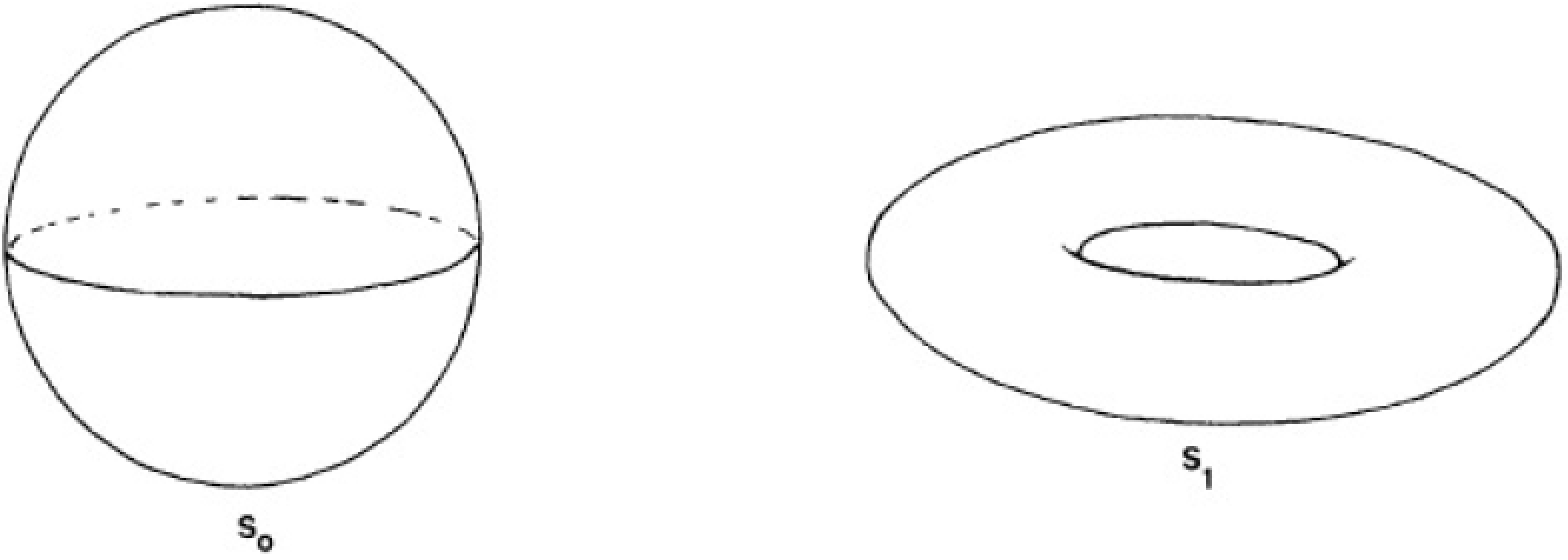
\includegraphics[width=0.35\textwidth]{../images/genus1.png} \quad
	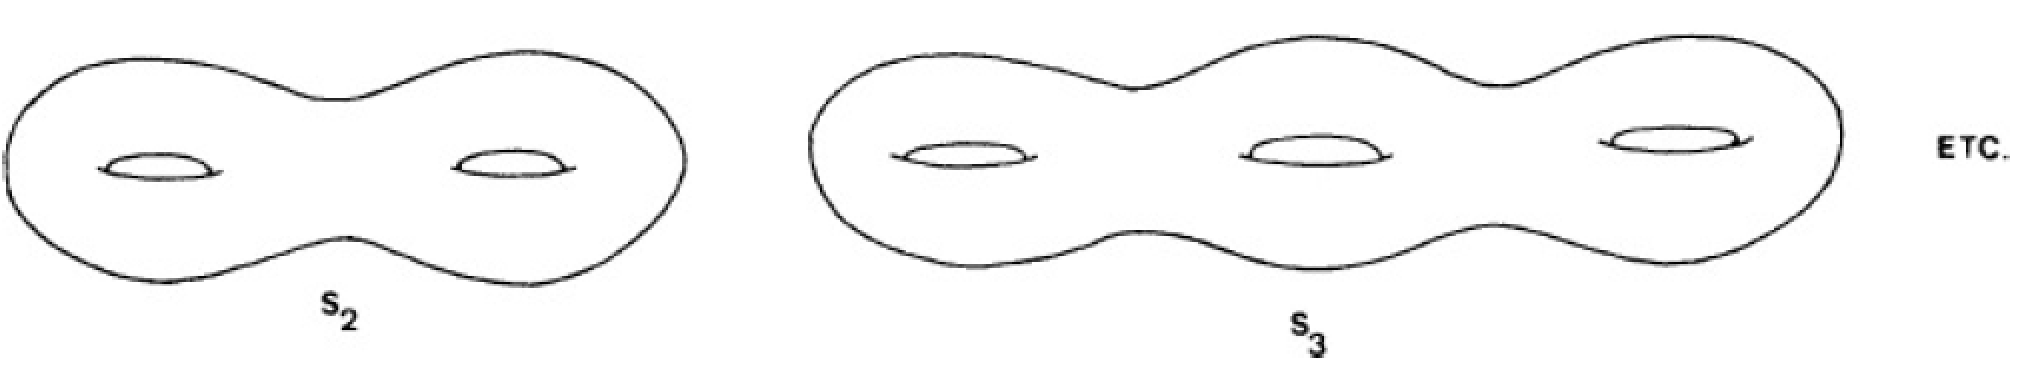
\includegraphics[width=0.45\textwidth]{../images/genus2.png}
	\end{figure}

\item {\bfseries Elliptic Curve.} An elliptic curve is\dots
	\begin{itemize}
	\item A nonsingular projective curve of genus 1.
	\item An abelian variety of dimension 1.
	\item A nonempty smooth variety, $V(F)$, with $\deg F=3$.
	\item A compact Riemann surface of genus 1.
	\item The set of solutions to\dots
	\[
	y^2 + a_1 xy + a_3y = x^3 + a_2 x^2 + a_4 x + a_6
	\]
along with a specified `distinguished point $\infty$' and an addition law given by the chord-tangent law.
	\end{itemize}

\item One can simply the last definition of an elliptic curve (called the Weierstrass form) to what is called the short Weierstrass form:
	\[
	y^2 + a_1 xy + a_3y = x^3 + a_2 x^2 + a_4 x + a_6
	\]  
	\begin{itemize}
	\item Make the substitution $y \mapsto y + \dfrac{a_1 x+a_3}{2}$.
	\item Obtain $y^2= x^3+ a_2' x^2 + a_4' x + a_6'$
	\item Make the substitution $x \mapsto x + \dfrac{a_2'}{3}$
	\end{itemize}  
	\[
	\star \enskip \boxed{E_{A,B}: y^2 = x^3 + Ax + B} \enskip \star
	\]

\item The set of rational points on an elliptic curve (ignoring the point at infinity) can be empty, finite, or infinite. 

\item {\bfseries CM (Complex Multiplication).} We say that an elliptic curve $E$ has complex multiplication (CM) or is CM if the endomorphism ring of $E$ is strictly larger than $\mathbb{Z}$. [The endomorphism ring, i.e. the ring of ring maps $E \to E$, always contains $\mathbb{Z}$ because we always have a map $E \to E$ give by multiplication by $n$, i.e. the map $P \mapsto nP$.]

\item {\bfseries $j$-invariant.} Take an elliptic curve $y^2= x^3 + Ax + B$. The transformations which preserve this equations are: $x= \mu^2 x$ and $y= \mu^3 y$ for $\mu \in \overline{K}^\times$. We then define the $j$-invariant
	\[
	j= 1728 \dfrac{4A^3}{4A^4 + 27B^2}
	\]
These classify elliptic curves up to isomorphism over $\overline{K}$.

\item {\bfseries Addition Law for Elliptic Curves.} To add two rational points on an elliptic curve (with the identity being the point at infinity and in short Weierstrass form), draw the line through the two points (or the tangent line in the case of a single distinct point) and find the intersection of the elliptic curve with this line (if the line is vertical the sum is the point at infinity). Reflect this point across the $x$-axis. This final point is the sum of the two rational points. By construction, it is immediate that this operation is abelian (you get the same line no matter the order of the points!). 
	\begin{figure}[h]
	\centering
	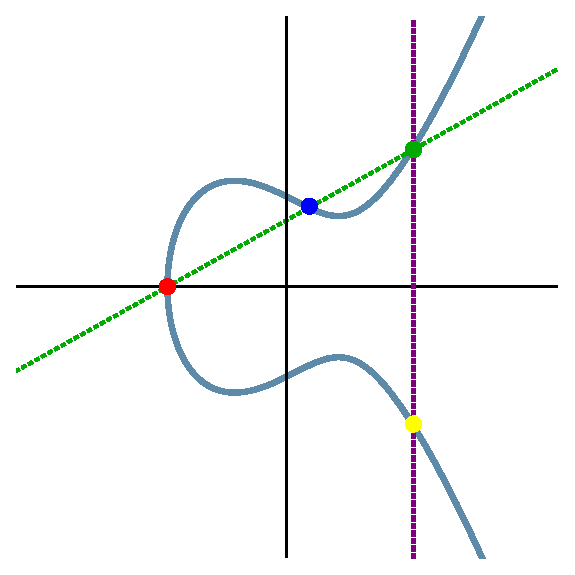
\includegraphics[width=0.25\textwidth]{../images/ec_add.eps}
	\end{figure}

\item {\bfseries Field.} A field is a collection of `numbers' where one can perform addition, subtraction, multiplication, and (nonzero) division and these operations are `nice.'

\item {\bfseries Galois Field.} A Galois field is a `number field' whose numbers satisfy extra symmetries. 

	\begin{thm*}[Mordell-Weil-N\'eron, 1952]
	Let $K$ be a field that is finitely generated over its prime field, and let $A/K$ be an abelian variety. Then the group of $K$-rational points on $A$, denoted $A(K)$, is a finitely generated abelian group. In particular,
		\[
		A(K) \cong \Z^{r_K} \oplus A(K)_{\text{tors}},
		\]
	where $r_K \geq 0$ is the rank and $A(K)_{\text{tors}}$ is the torsion subgroup. 
	\end{thm*}

\item By the above, every elliptic curve is isomorphic to a group of the form $\mathbb{Z}^r \oplus E_{\text{tors}}$, where $r$ is the rank of $E$ and $E_{\text{tors}}$ is the torsion subgroup. In fact, every elliptic curve is isomorphic to a group of the form\dots
	\[
	E \cong \Z^r \oplus \big(\Z/m\Z \oplus \Z/nm\Z \big)
	\]
for some $r, n, m$. 

\item The largest known rank for an elliptic curve is 28 due to Noam Elkies. It is known that 50\% of elliptic curves have rank 0 and 50\% have rank 1. `Most' elliptic curves are torsion-free, meaning the only point of finite order on $E$ is the identity. 

\item The collection of all points of order dividing $n$ over $\mathbb{C}$ on $E$ is denoted $E[n]$. In fact, $E[n] \cong \Z/n\Z \oplus \Z/n\Z$.

\begin{thm*}[Levi-Ogg Conjecture; Mazur, 1977]
If $E/\Q$ is a rational elliptic curve, then the possible torsion subgroups $E(\Q)_{\text{tors}}$ are precisely:
	\[
	\begin{cases}
	\Z/n\Z, & \text{with } n=1,2,\ldots,10,12 \text{ or} \\
	\Z/2\Z \oplus \Z/2n\Z, & \text{with } n=1,\ldots,4
	\end{cases}
	\]
Furthermore, each possibility occurs infinitely often.
\end{thm*}

\item {\bfseries Isogeny.} Let $E_1,E_2$ be elliptic curves. An isogeny from $E_1$ to $E_2$ is a morphism $\phi: E_1 \to E_2$ with $\phi(\mathcal{O})=\mathcal{O}$. If $|\ker \phi|=n$, we say $\phi$ is an $n$-isogeny. 

	\begin{thm*}[Fricke, Kenku, Klein, Kubert, Ligozat, Mazur, Ogg, et al.]
	If $E/\Q$ has an $n$-isogeny over $\Q$, then 
		\[
		n \in \{1,2,\ldots,19,21,25,27,37,43,67,163\}. 
		\]
	If $E$ does not have CM, then $n \leq 18$ or $n \in \{21,25,37\}$. 
	\end{thm*}
\end{itemize}



















\end{document}